\documentclass[ignorenonframetext,]{beamer}
\setbeamertemplate{caption}[numbered]
\setbeamertemplate{caption label separator}{: }
\setbeamercolor{caption name}{fg=normal text.fg}
\beamertemplatenavigationsymbolsempty
\usepackage{lmodern}
\usepackage{amssymb,amsmath}
\usepackage{ifxetex,ifluatex}
\usepackage{fixltx2e} % provides \textsubscript
\ifnum 0\ifxetex 1\fi\ifluatex 1\fi=0 % if pdftex
  \usepackage[T1]{fontenc}
  \usepackage[utf8]{inputenc}
\else % if luatex or xelatex
  \ifxetex
    \usepackage{mathspec}
  \else
    \usepackage{fontspec}
  \fi
  \defaultfontfeatures{Ligatures=TeX,Scale=MatchLowercase}
\fi
% use upquote if available, for straight quotes in verbatim environments
\IfFileExists{upquote.sty}{\usepackage{upquote}}{}
% use microtype if available
\IfFileExists{microtype.sty}{%
\usepackage{microtype}
\UseMicrotypeSet[protrusion]{basicmath} % disable protrusion for tt fonts
}{}
\newif\ifbibliography
\hypersetup{
            pdftitle={Lecture 13: Clustered Data, An Introduction to Applied Mixed Models},
            pdfauthor={Nick Reich / Transcribed by Gregory Guranich, edited by Bing Miu},
            pdfborder={0 0 0},
            breaklinks=true}
\urlstyle{same}  % don't use monospace font for urls
\usepackage{graphicx,grffile}
\makeatletter
\def\maxwidth{\ifdim\Gin@nat@width>\linewidth\linewidth\else\Gin@nat@width\fi}
\def\maxheight{\ifdim\Gin@nat@height>\textheight0.8\textheight\else\Gin@nat@height\fi}
\makeatother
% Scale images if necessary, so that they will not overflow the page
% margins by default, and it is still possible to overwrite the defaults
% using explicit options in \includegraphics[width, height, ...]{}
\setkeys{Gin}{width=\maxwidth,height=\maxheight,keepaspectratio}

% Prevent slide breaks in the middle of a paragraph:
\widowpenalties 1 10000
\raggedbottom

\AtBeginPart{
  \let\insertpartnumber\relax
  \let\partname\relax
  \frame{\partpage}
}
\AtBeginSection{
  \ifbibliography
  \else
    \let\insertsectionnumber\relax
    \let\sectionname\relax
    \frame{\sectionpage}
  \fi
}
\AtBeginSubsection{
  \let\insertsubsectionnumber\relax
  \let\subsectionname\relax
  \frame{\subsectionpage}
}

\setlength{\parindent}{0pt}
\setlength{\parskip}{6pt plus 2pt minus 1pt}
\setlength{\emergencystretch}{3em}  % prevent overfull lines
\providecommand{\tightlist}{%
  \setlength{\itemsep}{0pt}\setlength{\parskip}{0pt}}
\setcounter{secnumdepth}{0}
%       ************************************************
%       **        LaTeX preamble to be used with all 
%	**        statsTeachR labs/handouts.
%
%	Author: Nicholas G Reich
%	Last modified: July 2017
%	************************************************

%\documentclass[table]{beamer}

%	Set theme (a nice plain one)
\usetheme{Malmoe}

%	Use named colors, set main color of theme
%		to match Web site color:
\definecolor{MainColor}{RGB}{10, 74, 109}
\colorlet{MainColorMedium}{MainColor!50}
\colorlet{MainColorLight}{MainColor!20}
\usecolortheme[named=MainColor]{structure} 

%	For tables
%[dvipsnames] [table]
\usepackage{xcolor}

%% calling tabu.sty, assuming a particular directory structure
\usepackage{../../slide-includes/tabu}	% Even fancier than tabulary
\usepackage{multirow}

%	Just for the degree symbol
\usepackage{textcomp}

%	Get rid of footline (page, author, etc. on each slide)
\setbeamertemplate{footline}{}
%	Get rid of navigation buttons
\setbeamertemplate{navigation symbols}{}

%	Make footnotes not ugly
\usepackage{hanging}
\setbeamertemplate{footnote}{\raggedright\hangpara{1em}{1}\makebox[1em][l]{\insertfootnotemark}\footnotesize\insertfootnotetext\par}

%	Text style for code snippets inline in text:
\newcommand{\codeInline}[1]{\texttt{#1}}

%	Text style for emphasis stronger than \emph:
%		(Note, this doesn't toggle the way \emph does.
%			(Note, this can be done, didn't seem worth the trouble.))
\newcommand{\strong}[1]{{\bfseries{#1}}}


%        ******	Define title page	**********************
\setbeamertemplate{title page}{
	{\color{MainColor}
	% There must be a better way than this -vspace at
	%	 the top and bottom of the page to reduce the 
	%	 bottom margin, but I can't find one that works.
	%\vspace{-6em}

% 	% Go to a lot of trouble to get the title in a
% 	%	nice box, since customizing a beamer block
% 	%	does not entirely work here (I don't know why)
	\newlength{\titleBoxWidth}
	\setlength{\titleBoxWidth}{\textwidth}
	\addtolength{\titleBoxWidth}{-2.0em}
	\setlength{\fboxsep}{1.0em}
	\setlength{\fboxrule}{0pt}
	\fcolorbox{MainColor!25}{MainColor!25}{
		\parbox{\titleBoxWidth}{
			\raggedright
			\LARGE\textbf{\inserttitle}
		}	% end parbox
	}	% end fcolorbox

	\vfill
	\small{Author: \insertauthor}
	\vspace{\baselineskip}

	\small{Course: \underline{\href{http://nickreich.github.io/cda}{Categorical Data Analysis}} (BIOSTATS 743)}

%	\small{\Instructor}
%	\vspace{\baselineskip}

%	\small{\emph{This material is part of the \strong{statsTeachR} project}}

	\vfill
	
	\tiny{\emph{Made available under the \underline{\href{http://creativecommons.org/licenses/by-sa/4.0/}{Creative Commons Attribution-ShareAlike 4.0 International License}.}} \hfill \includegraphics[height=1em]{../../slide-includes/by-sa-compact.png}
 }


		\vspace{-15em}

	}	% end color
	\clearpage
}	% end define title page

\input{../../slide-includes/shortcuts}

\hypersetup{colorlinks,linkcolor=,urlcolor=MainColor}

\title{Lecture 13: Clustered Data, An Introduction to Applied Mixed Models}
\author{Nick Reich / Transcribed by Gregory Guranich, edited by Bing Miu}
\date{}

\begin{document}
\frame{\titlepage}

\begin{frame}{Clustered Data}

\begin{itemize}
\tightlist
\item
  \textbf{Clustered Data:}\\
\item
  Hierarchy, nested populations\\
\item
  Longitudinal, Correlated observations or sets .eg repeated measure
\item
  \textbf{Example: (Hierarchy of nested populations)}\\
\item
  Patient \(\in\) Hospital \(\in\) Region 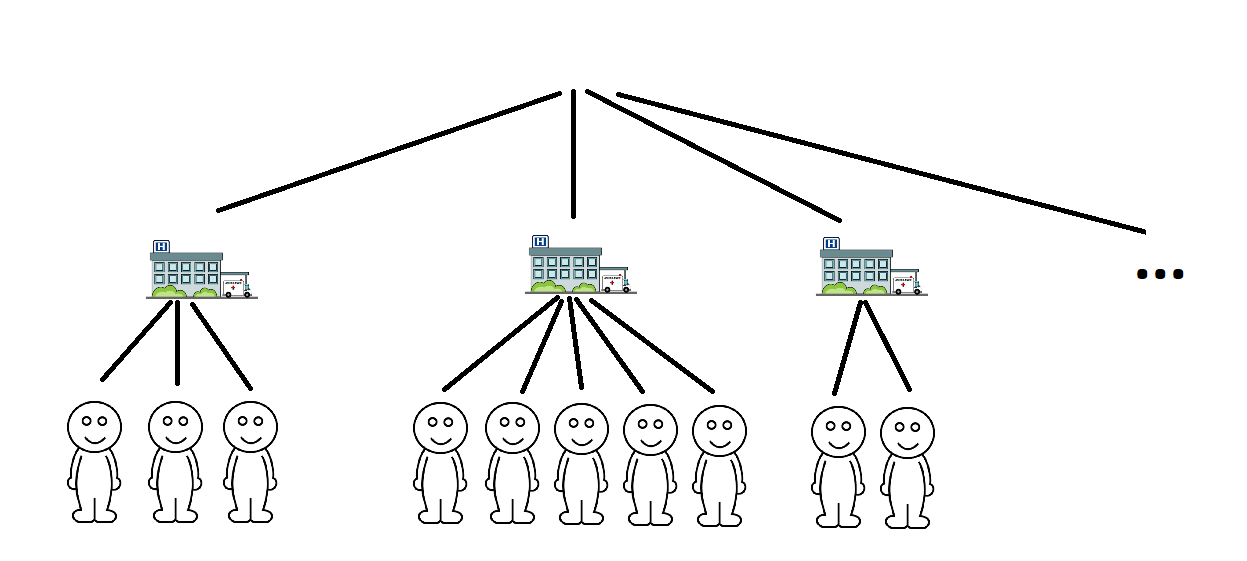
\includegraphics{img1.png}
\end{itemize}

\end{frame}

\begin{frame}{Clustered Data}

\begin{itemize}
\tightlist
\item
  \textbf{Example: (Longitudinal)}
\item
  Repeated measurements on the same unit of observation

  \begin{itemize}
  \tiny
  \item Patients have multiple temperature measurements over time
  \item Temperature $\in$ Patient $\in$ Clinic
  \end{itemize}
\end{itemize}

\begin{figure}
\centering
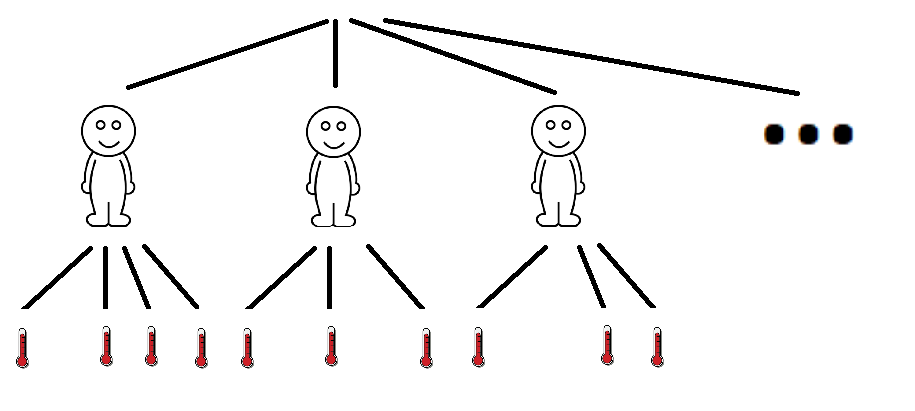
\includegraphics{img2.png}
\caption{Alkema 2017}
\end{figure}

\end{frame}

\begin{frame}{Implications of Clustered Data}

\begin{itemize}
\tightlist
\item
  Observations in clusters violates our assumptions of independence
\item
  Clustered data are less informative and less generalizable than
  independent data
\item
  \textbf{Example:} Subjects within a household are more similar and
  will vary less. Similar genetics and behavior
  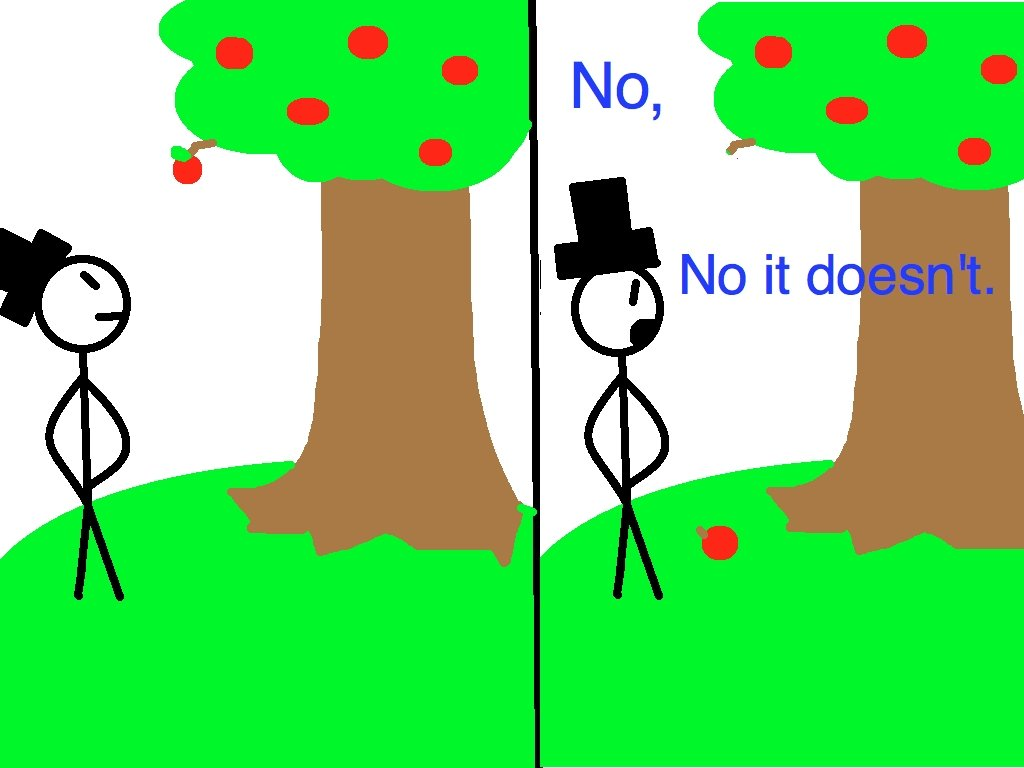
\includegraphics{img3.jpg}
\end{itemize}

\end{frame}

\begin{frame}{Example Notation}

Mixed models, also known as multilevel or hierarchical models, are used
to model cluster data. We will use the following notation to model such
data.

\(Y_{ij} =\) Response variable

\(Trt_{ij} =\) Treatment variable

\end{frame}

\begin{frame}{Example Notation 2}

\[j = 1,~2,~...,~n\] \[i = 1,~2,~...,~n_i\]
\[N = \sum_i n_i= \text{total number of groups}\]
\[Treatment ~~Trt_{ij} = \begin{cases} 1, & \mbox{if $Trt_{ij}$ was treated} \\ 0, & \mbox{otherwise } \end{cases}\]

\begin{figure}
\centering
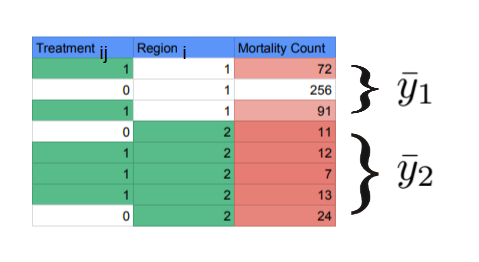
\includegraphics[width=3.90625in]{img5.png}
\caption{}
\end{figure}

\end{frame}

\begin{frame}{Example to begin with}

\begin{itemize}
\item
  Let \(Y_{ij}\) denotes the counts of mortality
  \[Y_{ij} \sim Poisson(\lambda_{ij},P_{i})\]
  \[log(\lambda_{ij}) = \beta_0 + \beta_1Trt_{ij} + \beta_2X_i\]
\item
  We want to make inference about \(\beta_1\). What is the treatment
  effect?\\
\item
  Observations are not iid, need ``adjustment''
\item
  How can we account for variance within groups? \small

  \begin{itemize}
  \item 1. Marginal models with generalized estimating equations (GEE) for variance adjustment 
  \item 2. generalized linear mixed models (GLMM's)
  \end{itemize}
\end{itemize}

\end{frame}

\begin{frame}{GLMM's Models}

\begin{itemize}
\tightlist
\item
  Account for modeling for individual and group level variation in
  estimating group-level coefficients
\item
  Allow the proper measure of variation in individual level regression
  coefficients
\item
  For point estimates, Shrinkage (relative to sample size) of parameters
  toward group means
\item
  Rule of thumb \small

  \begin{itemize}
  \item number of groups greater than 5
  \item substainial variation among groups
  \end{itemize}
\end{itemize}

\end{frame}

\begin{frame}{GLMMS Model Notation}

\begin{itemize}
\item
  where \(\beta\) is a fixed effect and \(\mu_i\) are varying (random)
  effects \[
  \begin{aligned}
  g(E[y_{ij}|\mu_i]) = X^T_{ij}\beta + Z^T_{ij}\mu_i \\
  \mu_{i} \sim N(0, G_\theta)
  \end{aligned}
  \]
\item
  Agresti uses \emph{i} to represent the group, \(Y_{ij}\) is the
  \(jth\) observation in \(ith\) group
\item
  So here we have \emph{i} different \(\mu\) which are draws from a
  normal
\item
  The \(\mu_i\) have a common distribution
\item
  Notice \(\beta\) has no subscript, \(\beta\) is fixed
\item
  \(\beta\) is a global estimate and \(\mu_i\) is a group specific
  estimate
\item
  \(g\) is a glm link
\item
  \(\theta\) is a parameter that governs the distribution of the random
  effect
\end{itemize}

\end{frame}

\begin{frame}{Estimation}

\[
\begin{aligned}
L(\beta,\theta) &=f(\vec y|\beta, \theta)\\
&= \int f(\vec{y} |\vec\mu)f(\vec\mu)du
\end{aligned}
\]

\begin{itemize}
\tightlist
\item
  where we integrate across our marginal \(f(\hat\mu)\)
\item
  these problems usually do not have closed form solutions
\item
  How to approximate? Use Bayesian MCMC or HMC algorithims to sample
  from posterior distribution of \(\beta\) and \(\theta\)
\item
  approximate with Laplace methods (some coefficients are subject to
  penalty terms)
\item
  \textbf{Degrees of Freedom:} Approximated by estension of the Hat
  matrix \small

  \begin{itemize}
  \item some closed for solutions (ex: beta-binomial conjugate in next lecture)
  \end{itemize}
\end{itemize}

\[
\begin{aligned}
tr(H) = p \\
p \leq tr(H) \leq p
+q
\end{aligned}
\]

\end{frame}

\begin{frame}{Example}

\begin{itemize}
\tightlist
\item
  Lets say we are looking at treatment(spinal implants) to relieve back
  pain. Rows represent visit 1 and columns represent visit 2
\end{itemize}

\begin{figure}
\centering
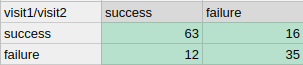
\includegraphics[width=2.60417in]{img6.png}
\caption{}
\end{figure}

\begin{itemize}
\tightlist
\item
  pain indicator \(Y_{ij}\) and group indicator \(X_{ij}\)
  \[y_{ij} = \begin{cases}
  1 & \text{ patient j at visit i has no pain} \\
  0 & \text{ patient j at visit i has pain}
   \end{cases}\]
\end{itemize}

\[x_{ij} = \begin{cases}
    1 & \text{i=2; patient's second visit} \\
    0 & \text{i=1; pateint's first visit}
 \end{cases}\]

\end{frame}

\begin{frame}{Example (possible models)}

\begin{itemize}
\tightlist
\item
  logistic-normal model
\end{itemize}

\[
\begin{aligned}
logit(P(Y_{ij}=1|\mu_i)) = \alpha + \beta X_{ij} + \mu_i \\
\mu_i \sim N(0, \sigma^2_{\mu})
\end{aligned}
\]

\begin{itemize}
\tightlist
\item
  logistic-normal, similar notation for bayesians with weakly
  informative priors
\end{itemize}

\[
\begin{aligned}
Y_i \sim N(\pi, \sigma^2_y) \\
logit(\pi) = \alpha_i + \beta X_{ij}\\
\alpha_i \sim N(\beta_0, \sigma^2_\alpha) \\
\beta_0 \sim N(0,100)\\
\sigma_\alpha \sim U(0,5)
\end{aligned}
\]

\end{frame}

\begin{frame}{Example (interpretation)}

\[
\begin{aligned}
logit(P(Y_{ij}=1|\mu_i)) = \alpha + \beta X_{ij} + \mu_i \\
\mu_i \sim N(0, \sigma^2_{\mu})
\end{aligned}
\]

\begin{itemize}
\tightlist
\item
  \(\alpha \sim\) log odds of pain free at visit 1
\item
  \(\beta \sim\) change in log odds of being pain free comparing visit 2
  to visit 1
\end{itemize}

\end{frame}

\begin{frame}{Example (interpretation)}

\begin{itemize}
\tightlist
\item
  With mixed effect \(\mu_i\) our intercept can now vary
  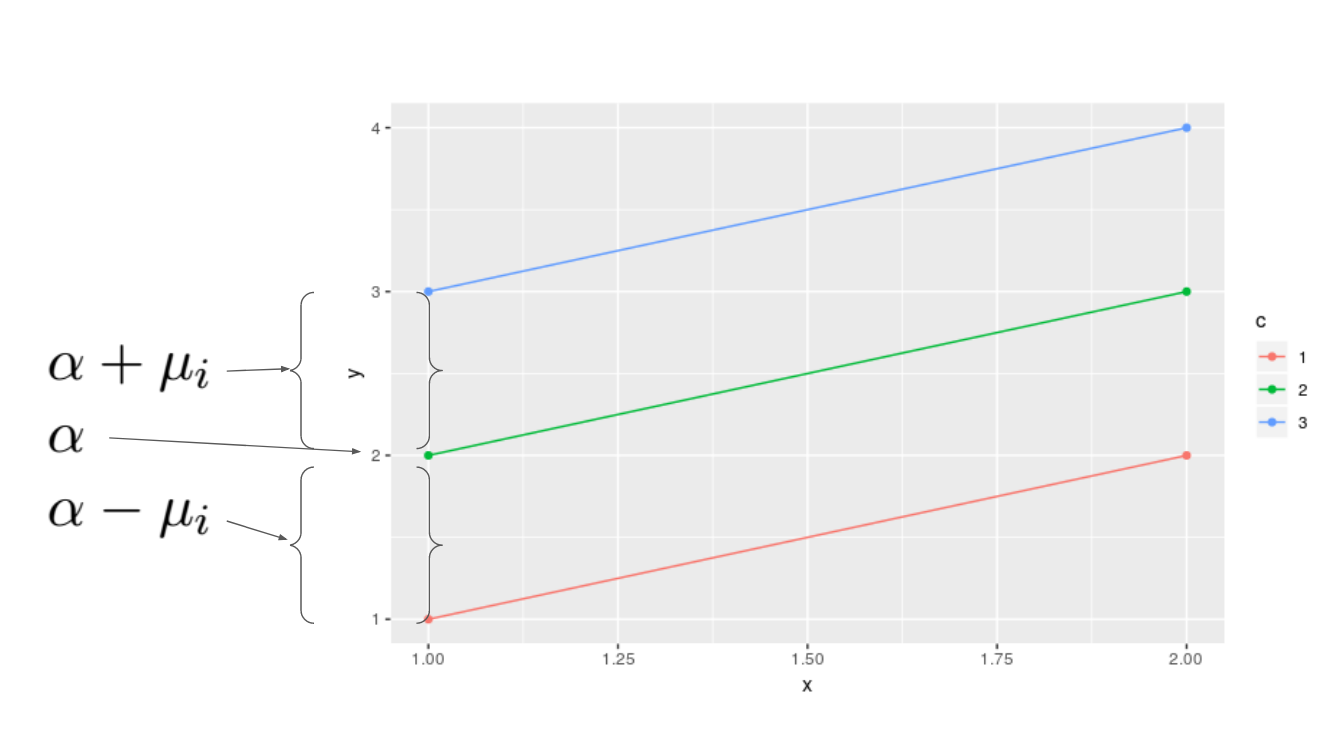
\includegraphics[width=4.16667in]{img_mixed.png}
\end{itemize}

\end{frame}

\end{document}
